\documentclass{emulateapj}
\submitted{{\it Submitted for publication in ApJ}}
\usepackage{multirow,color,wrapfig,ulem}
\usepackage {graphicx}
\usepackage{graphics}
\usepackage[dvips]{epsfig}

%=========================================================================
%		INTERNAL MACROS
%=========================================================================
\def\be{\begin{equation}}
\def\ee{\end{equation}}
\def\ba{\begin{eqnarray}}
\def\ea{\end{eqnarray}}

% To highlight comments 
\definecolor{red}{rgb}{1,0.0,0.0}
\newcommand{\red}{\color{red}}
\definecolor{darkgreen}{rgb}{0.0,0.5,0.0}
\newcommand{\SRK}[1]{\textcolor{darkgreen}{\bf SRK: \textit{#1}}}
\newcommand{\SRKED}[1]{\textcolor{darkgreen}{\bf #1}}
\newcommand{\before}[1]{\textcolor{red}{ #1}}
\newcommand{\after}[1]{\textcolor{darkgreen}{ #1}}

\newcommand{\LCDM}{$\Lambda$CDM~}
\newcommand{\beq}{\begin{eqnarray}}  
\newcommand{\eeq}{\end{eqnarray}}  
\newcommand{\zz}{$z\sim 3$} 
\newcommand{\avg}[1]{\langle{#1}\rangle}  
\newcommand{\ly}{{\ifmmode{{\rm Ly}\alpha}\else{Ly$\alpha$}\fi}}
\newcommand{\hMpc}{{\ifmmode{h^{-1}{\rm Mpc}}\else{$h^{-1}$Mpc}\fi}}  
\newcommand{\hGpc}{{\ifmmode{h^{-1}{\rm Gpc}}\else{$h^{-1}$Gpc}\fi}}  
\newcommand{\hmpc}{{\ifmmode{h^{-1}{\rm Mpc}}\else{$h^{-1}$Mpc}\fi}}  
\newcommand{\hkpc}{{\ifmmode{h^{-1}{\rm kpc}}\else{$h^{-1}$kpc}\fi}}  
\newcommand{\hMsun}{{\ifmmode{h^{-1}{\rm {M_{\odot}}}}\else{$h^{-1}{\rm{M_{\odot}}}$}\fi}}  
\newcommand{\Mmin}{{\ifmmode{{M_{\rm min}}}\else{${M_{\rm min}}$}\fi}}
\newcommand{\mmin}{{\ifmmode{{M_{\rm min}}}\else{${M_{\rm min}}$}\fi}}
\newcommand{\mmax}{{\ifmmode{{M_{\rm max}}}\else{${M_{\rm max}}$}\fi}}
\newcommand{\lmmin}{{\ifmmode{{\log M_{\rm min}}}\else{${\log M_{\rm min}}$}\fi}}
\newcommand{\lmmax}{{\ifmmode{{\log M_{\rm max}}}\else{${\log M_{\rm max}}$}\fi}}

\newcommand{\Mmax}{{\ifmmode{{M_{\rm max}}}\else{${M_{\rm max}}$}\fi}}
\newcommand{\dm}{{\ifmmode{{\Delta M}}\else{$\Delta M$}\fi}}
\newcommand{\dlm}{{\ifmmode{{\Delta \log M}}\else{$\Delta \log M$}\fi}}
\newcommand{\focc}{{\ifmmode{{f_{\rm occ}}}\else{${f_{\rm occ}}$}\fi}}

\newcommand{\Msun}{{\ifmmode{{\rm {M_{\odot}}}}\else{${\rm{M_{\odot}}}$}\fi}}  
\newcommand{\msun}{{\ifmmode{{\rm {M_{\odot}}}}\else{${\rm{M_{\odot}}}$}\fi}}  
\newcommand{\lya}{{Lyman$\alpha$~}}
\newcommand{\clara}{{\texttt{CLARA}}~}
\newcommand{\rand}{{\ifmmode{{\mathcal{R}}}\else{${\mathcal{R}}$ }\fi}}  
%SAMPLES


%MY COMMANDS #############################################################
\newcommand{\sub}[1]{\mbox{\scriptsize{#1}}}
\newcommand{\dtot}[2]{ \frac{ d #1 }{d #2} }
\newcommand{\dpar}[2]{ \frac{ \partial #1 }{\partial #2} }
\newcommand{\pr}[1]{ \left( #1 \right) }
\newcommand{\corc}[1]{ \left[ #1 \right] }
\newcommand{\lla}[1]{ \left\{ #1 \right\} }
\newcommand{\bds}[1]{\boldsymbol{ #1 }}
\newcommand{\oiint}{\displaystyle\bigcirc\!\!\!\!\!\!\!\!\int\!\!\!\!\!\int}
\newcommand{\mathsize}[2]{\mbox{\fontsize{#1}{#1}\selectfont $#2$}}
\newcommand{\eq}[2]{\begin{equation} \label{eq:#1} #2 \end{equation}}
\newcommand{\lth}{$\lambda_{th}$ }
\newcommand{\reff}{{\ifmmode{r_{\mbox{\tiny eff}}}\else{$r_{\mbox{\tiny eff}}$}\fi}}
%#########################################################################

%TO DO COMMANDS. Highlight region that needs extra work  #############################################################
\newcommand{\todo}{\ifmmode \text{\Huge{\(\bullet\)}} \else {\Huge$\bullet$}\fi}
% \newcommand{\todo}{\ifmmode {\Huge \bullet} \else {\Huge$\bullet$}\fi}
\newcommand{\tido}{\ifmmode {\bullet} \else $\bullet$\fi}
\newcommand{\REFS}{(\todo REFS) }
\newcommand{\toref}{(\todo REFS)}
%#########################################################################



\begin{document}
%=========================================================================
%		FRONT MATTER
%=========================================================================
\title{Uncertainty on the galaxy-halo connection for Lyman-$\alpha$ emitters at $z=3.1$}
\author{
  Juli\'an E. Mej\'ia-Restrepo \thanks{jemejia@das.uchile.cl}$^{1,3}$,
  Jaime E. Forero-Romero \thanks{je.forero@uniandes.edu.co}$^{2}$ 
}

\affil{
$^1$Departamento de Astronom\'{i}a, Universidad de Chile, Camino el Observatorio 1515, Santiago, Chile\\
$^2$Departamento de F\'{i}sica, Universidad de los Andes, Cra. 1
No. 18A-10, Edificio Ip, Bogot\'a, Colombia\\
$^3$FACom-Instituto de F\'isica-FCEN, Universidad de Antioquia, Calle 70 No. 52-21, Medell\'in, Colombia
}





\begin{abstract}
We study the impact of cosmic variance and observational uncertainties
in constraining the mass and occupation fraction, \focc, of
dark matter halos hosting \ly\ Emitting  Galaxies (LAEs) at high redshift. 
We construct mock catalogs from an N-body simulation to match the 
typical size of observed fields at $z=3.1$ ($\sim 1 {\rm deg^2}$).
In our model a dark matter halo with mass in the range $\mmin
<M_{\mathrm h}<\mmax$ can only host one detectable LAEat most.    
We explore the parameter space determined by \mmin, \mmax\ and \focc\
with a Markov Chain Monte-Carlo algorithm using as observational
constraints the angular correlation function (ACF) and the LAEs number density. 
We find that the preferred minium and maximum masses in our model span
a wide range $10^{9.6}\hMsun\leq \mmin \leq 10^{11.0}\hMsun$ ,
$10^{10.9}\hMsun\leq \mmax \leq 10^{13.0}\hMsun$; followed by a
wide range in the occupation fraction $0.02\leq \focc \leq 0.30$.   
As a consequence the median mass, $M_{50}$, of all models consistent with
observations has a large uncertainty $M_{50} =
3.16^{+9.34}_{-2.37}\times 10^{10}$\hMsun, in agreement with the most recent
observational estimates.
However, we find that the same individual models have a relatively tight
mass gap, $\Delta M \equiv \log_{10}\mmax - \log_{10}\mmin$, of $\Delta
M\approx 0.3$dex.
We are also able show that \focc\ is uniquely determined by $M_{\rm
  min}$, regardless of $M_{\rm max}$, by
$\focc\sim0.1(\mmin/10^{10.5}\hMsun )^{0.93}$.  
However, the current observational data only allows us to put weak
constraints on \mmin\ and consequently on \focc.
We show that upcoming large surveys covering at least $50$ deg$^{2}$
will be able to put tighter constraints on \mmin\ and \focc\ through the LAE number density
distribution width, $W_{1\sigma}$, constructed over several fields of
$\sim 1$ deg$^{2}$ using the relationship, $W_{1\sigma} =
0.138\times (\mmin/10^{11}\hMsun )^{0.177}$, calibrated from our results.
\end{abstract}

\keywords{
Cosmology: theory - large-scale structure of Universe -
Methods: data analysis - numerical - N-body simulations
}

%*************************************************************************
\section{Introduction}
\label{sec:introduction}
\toref ADD NEWER REFERENCES
Lyman-$\alpha$ emitting galaxies (LAEs) are central to a wide range
of subjects in extragalactic astronomy. 
LAEs can be used as probes of reionization \citep{Dijkstra11}, tracers
of large scale structure \citep{Koehler2007},  signposts for low
metallicity stellar populations, markers of the galaxy formation
process at high redshift \citep{Dayal2009,ForeroRomero2012} and
tracers of active star formation \citep{Guaita2013}.  

In most of those cases, capitalizing the observations requires
understanding how LAEs are formed within an explicit cosmological
context.  
Under the current structure formation paradigm the dominant matter
content of the Universe is dark matter (DM).  
Each galaxy is thought to be hosted by a larger dark matter structure
known as a halo. \citep{Peebles1980,SpringelNature05}.  
Understanding the cosmological context of LAEs thus implies studying
the galaxy-halo connection.  
Galaxy formation models suggest that the physical processes that regulate the star formation cycle are dependent on halo mass \citep[e.g.][]{Behroozi2013a}.
The mass becomes the most important element in the halo-galaxy connection. 
   
The goal becomes finding the typical DM halo mass of halos hosting LAEs.
In the case of LAEs there are different ways to find this mass range.
One approach is theoretical, using general astrophysical principles to
find the relationship between halo mass, intrinsic \ly\ luminosities
and observed \ly\ luminosities. This approach is usually implemented
through semi-analytic models \citep{Garel2012,Orsi2012} and  full
N-body hydrodynamical simulations \citep{Laursen2007, Dayal2009,
  ForeroRomero2011, Yajima2012}.  



The downside of these calculations is the uncertainty in the
estimation of the escape fraction of \ly\ photons. Given the resonant
nature of the \ly\ line, the escape fraction is sensitive to  the dust
contents, density, temperature, topology and kinematics of the neutral
Hydrogen in the interstellar medium (ISM). The process of finding a
consensus on the expected value for the \ly\ escape fraction in high
redshift galaxies is still matter of open debate
\citep{Neufeld1991,Verhamme2006,ForeroRomero2011,Dijkstra2012,Laursen2013,Orsi2012}. 

A different approach to infer the typical mass of halos hosting
LAEs is based on the spatial clustering information. 
This approach uses the fact
that in CDM cosmologies the spatial clustering of galaxies on large
scales is entirely dictated by the halo distribution
\citep{Colberg00}, which in turn has a strong dependence on halo
mass. 
Using measurements of the angular correlation function of LAEs,
observers have put constraints on the typical mass and occupation
fraction of the putative halos hosting these galaxies
\citep{Hayashino2004,Gawiser07,Nilsson2007,Ouchi2010,Bielby16}. 
In these studies the observations are done on fields of $\sim 1$ deg$^{2}$ and
the conclusions derived on the halo host mass do not elaborate on the
uncertainty resulting from the cosmic variance on these fields. 

In this letter we investigate the impact of cosmic variance in
constraining the mass and occupation fraction of halos hosting LAEs at $z=3$.
We build mock surveys from a cosmological N-body simulation to compare them
against the observations of \cite{Bielby16} using the angular
correlation function.  
We use a simple model to populate a halo in the simulation with a LAE   
assuming a minimum (\mmin) and maximum mass (\mmax) for the dark
matter halos hosting LAEs without predicting a \ly\  luminosity.  
This approach bypasses all the physical uncertainties associated to
star formation and radiative transfer. 
We use the Markov Chain Monte Carlo technique to obtain the likelihood
of the parameters given the observational constraints. 

Throughout this letter we assume a $\Lambda$CDM cosmology with the
following values for the cosmological parameters, $\Omega_{m}=0.30711$,
$\Omega_{\Lambda}=0.69289$ and $h=0.70$, corresponding to the matter
density, vacuum density and the Hubble constant in units of 100 km
s$^{-1}$ Mpc$^{-1}$. 


\begin{figure}
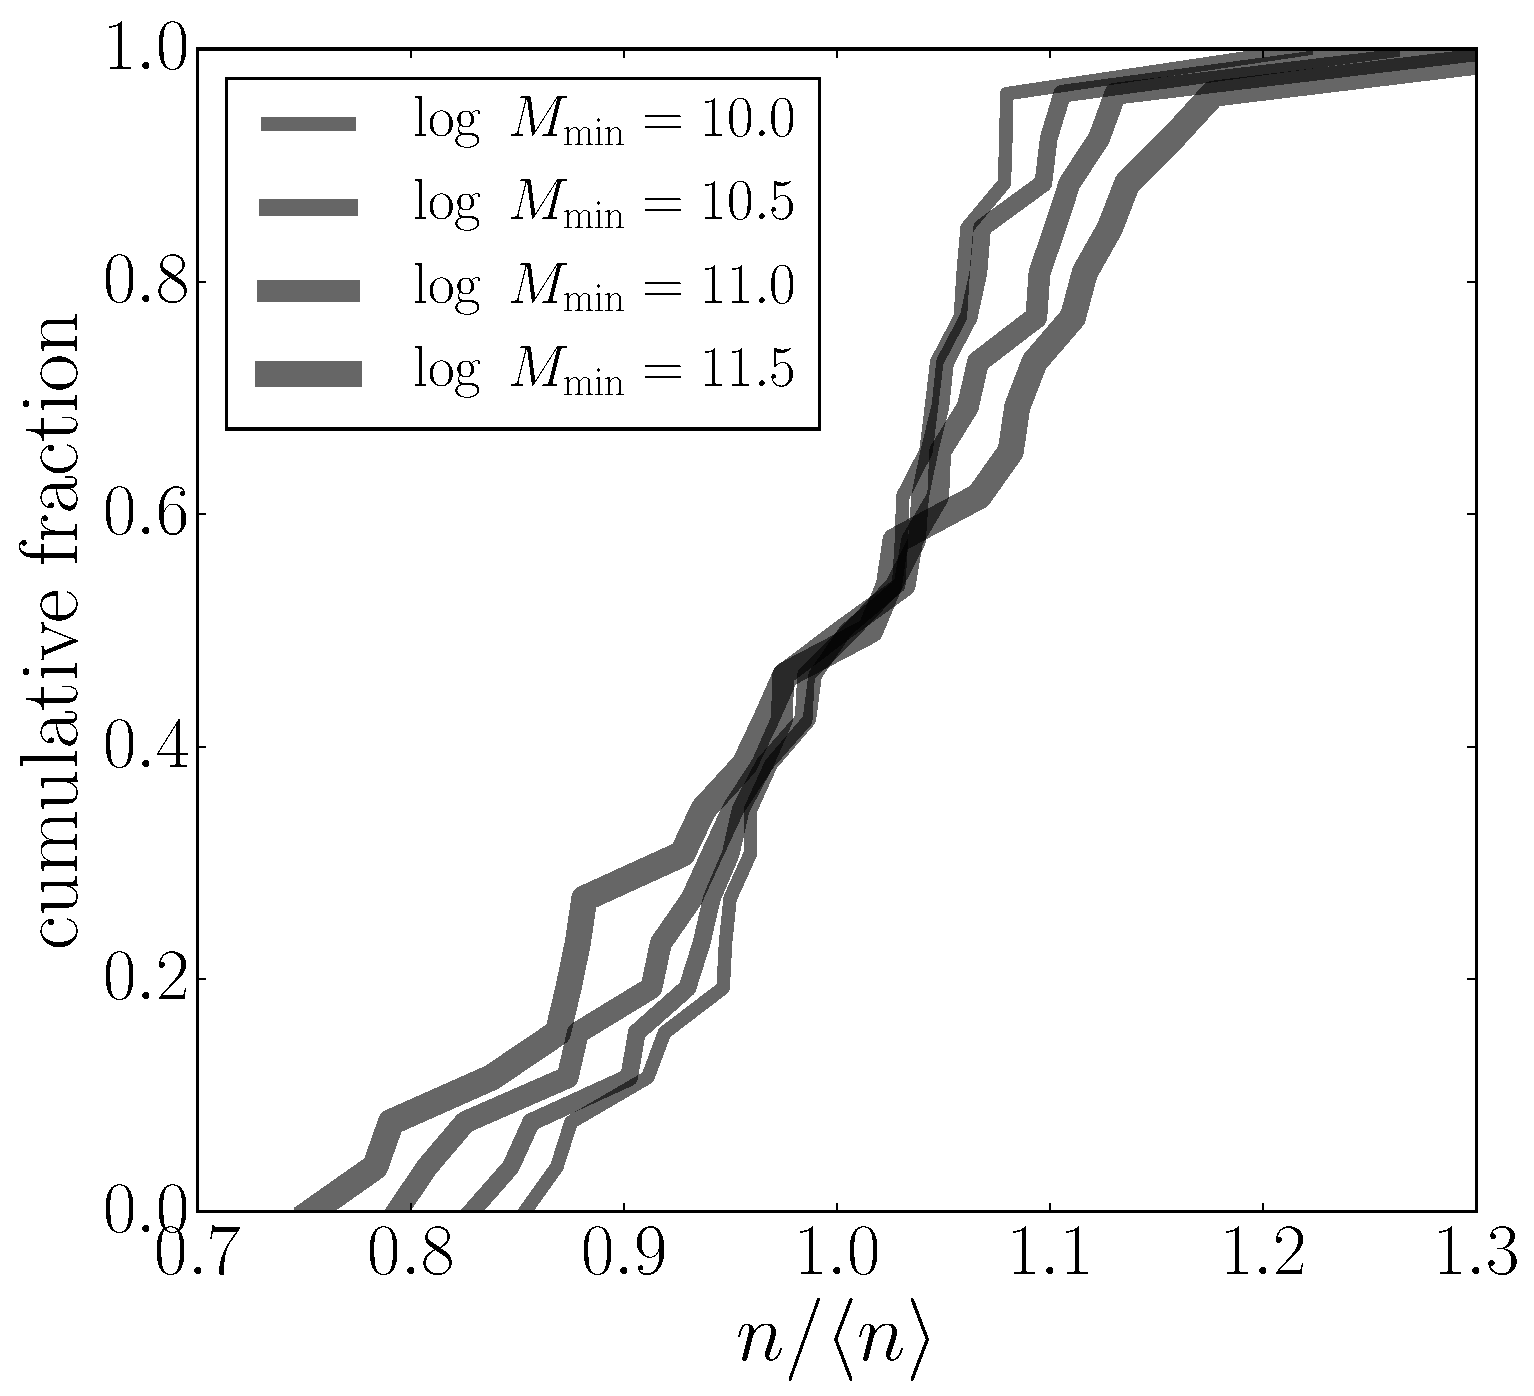
\includegraphics[width=0.47\textwidth]{fig1.pdf}
\caption{Cumulative halo number density distribution function over
  27 mock fields. Each line corresponds to a
  different model with increasig values of $M_{\rm min}$. 
  Different models produce different number density distributions. The
width of the distribution increases with \mmin. } 
\label{fig:cosmicv0}
\end{figure}




\section{Methodology}

The base of our method is the comparison between observations and mock
catalogs. 
This approach allows us to take explicitly into account cosmic variance. 
The comparison has four key elements. 
First, the observations we take as a benchmark. 
Second, the N-body simulation and the halo catalogs we use to build
the mocks. 
Third, the parameters describing our model to
assign a LAE to a halo. 
Fourth, the statistical method we adopt to compare observations and
simulations.  
We describe in detail these four elements in the following subsections.




\subsection{Observational constraints}
\label{subsec:obs}
\citet{Bielby16} used narrow band imaging to detect 643 LAE candidates
at $z\sim 3$  with equivalent widths of $\gtrsim$65\AA\ and a flux limit
of $2\times10^{17}{\rm erg/cm^2/s}$ ($L\sim 7\times10^{42}{\rm erg/s} $). 
Using spectroscopy they found a 22\% contamination fraction.
Their observations cover 5 (out of 9) independent and adjacent
fields of the VLT LBG Redshift Survey (VLRS).  
The  total observed  area corresponds to 1.07$\rm deg^2$ that translates to
$\sim$80$^2\hMpc^2$ in a comoving scale. 
\citet{Bielby16} used the NB497  narrow-band filter whose 77\AA\ FWHM
and 154\AA\ Full width  tenth maximum (FWTM) correspond to a total observational depth of
44\hMpc\  and 82\hMpc\ comoving, respectively. 

\begin{figure}
  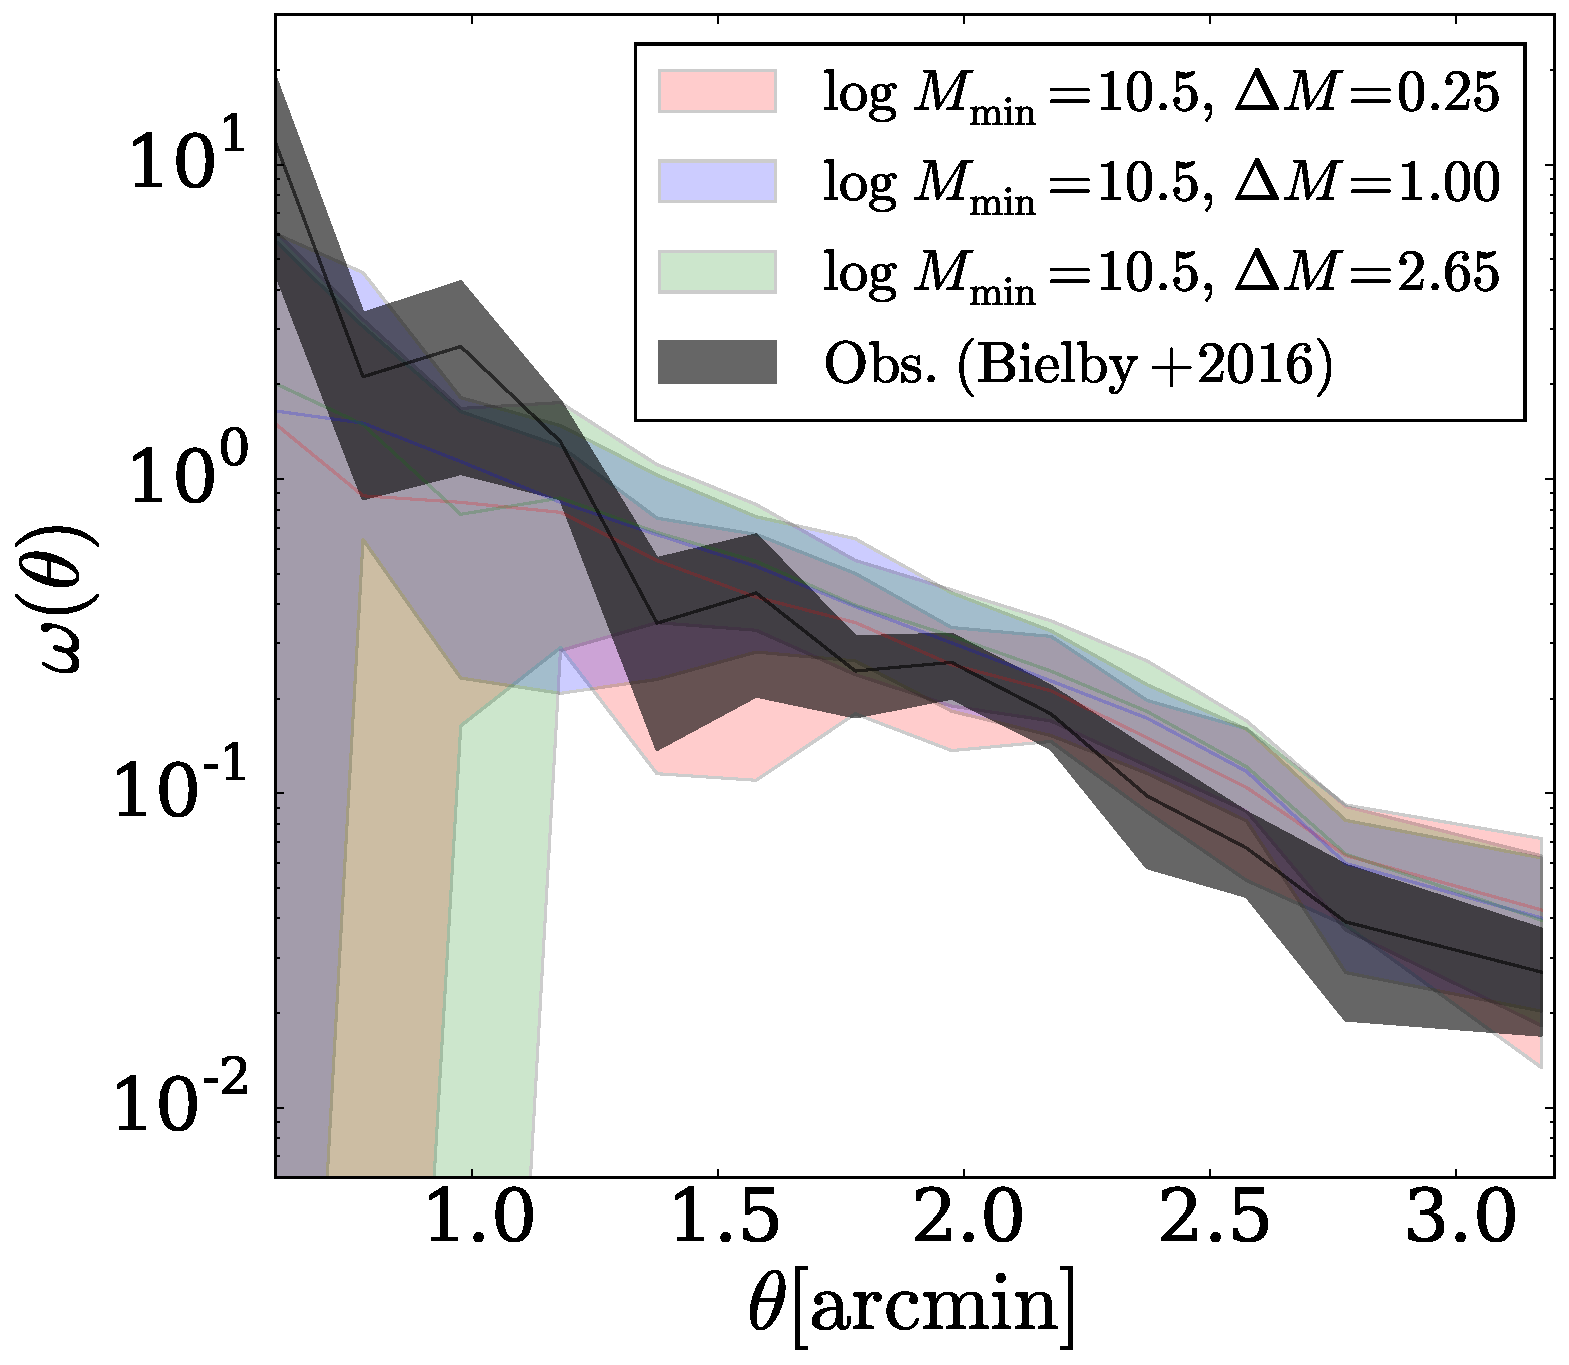
\includegraphics[width=0.47\textwidth]{fig5.pdf}
\caption{ Angular Correlation functions for $\log M_{\rm
    min}[\rm{M_{\odot}h^{-1}}]=10.5$ and different values of $\Delta \log
  M$.  
  The shaded region in the models represents the $1-\sigma$ variation
  due to cosmic variance. Radically different models in $\Delta \log M$ are consistent with
  observations once cosmic variance is modelled in detail.} 
\label{fig:corr}
\end{figure}


\subsection{Simulation and halo catalog}
\label{subsec:sim}

We use results from the Bolshoi simulation \citep{Bolshoi,BolshoiP} which was
performed in a cubic volume of 250 $h^{-1}$ Mpc comoving on a side. 
The dark matter distribution was sampled using  $2048^{3}$
particles. 
The cosmological parameters are consistent with Planck
results \citep{Planck2014} with a matter density 
$\Omega_{\rm m} = 0.307$, cosmological constant
$\Omega_{\Lambda}=0.693$, dimensionless Hubble constant $h=0.678$, slope
of the power spectrum  $n=0.96$ and normalization of the power
spectrum $\sigma_{8}=0.823$.  
This translates into a particle mass of  $m_{\rm p}=1.5\times 10^{8}$
$h^{-1}$ M$_{\odot}$.   


We use halo catalogs constructed with a Bound-Density-Maxima (BDM)
algorithm. 
The catalogs were obtained from the publicly available Multidark
database  \footnote{\url{http://www.multidark.org/MultiDark/}}
\citep{MultiDark}. 
For each  halo in the box we extract its comoving position and mass.  
We focus our work on halos more massive than $1.5\times
10^{9}$\hMsun\ resolved with at least  $10$ particles. 
We do not take into account sub-halos.


We split the simulation volume at z$\sim$3 into  27 smaller mock
volumes mimicking the  area and depth reported in \citet{Bielby16} and
described in \S \ref{subsec:obs}.   


\begin{figure*}
\begin{center}
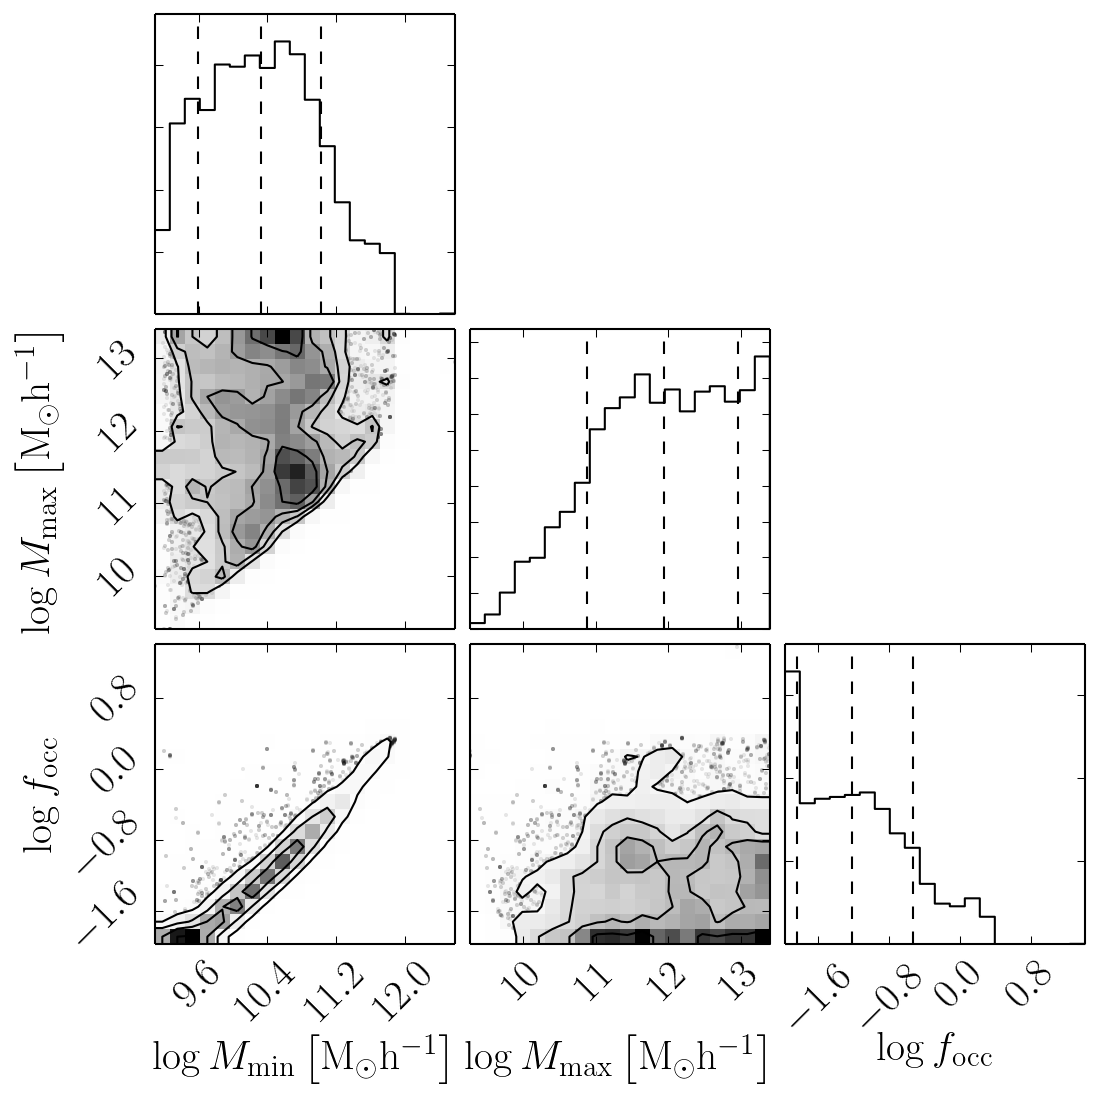
\includegraphics[width=0.85\textwidth]{likelyplot_1deg_total.png}
\end{center}
\caption{One and two dimensional projections of the posterior
  probability distributions of \mmin, \mmax\ and \focc\. 
  The models with $\log \focc>0.00$ ($\focc>1$) correspond  to models
  where the number density  of halos is smaller than the number of
  observed LAEs but we consider them as consistent because of the uncertainty
  in the median number density due to cosmic variance. See 
Fig. \ref{fig:cosmicv0} and \S\ref{subsec:explore} for details.} 
\label{fig:like}
\end{figure*}


\subsection{A simple LAE model}
\label{subsec:mocks}

We build the simplest possible model to assign a LAE to each DM halo
without trying to compute a LAE luminosity.
  
We first assume that a dark matter halo can host one detectable LAE at
most.   
This assumption is consistent with theoretical analysis of the
correlation function \citep{Jose2013b} and observations that confirm a
lack of class pairs in LAEs \cite{Bond2009}.  
Then we say that a halo will host a LAE with probability $\focc$
if and only if the halo mass is in the range $\mmin < M_{\mathrm
  h} < \mmax$. 
We also use the variable \dlm to represent the mass range width,
$\dlm\equiv\ \log \mmax - \log \mmax$.  


The parameter $\focc$ can be thought as the LAE occupation fraction of
dark matter halos.
An astrophysical interpretation of $f_{\rm occ}$ convolves at least
three phenomena: the actual presence of a star forming galaxy in a
halo, the escape fraction of \ly\ radiation and its detectability as
a LAE.   
We do not try to disentangle these complex phenomena.
We instead opt for an arithmetic interpretation by setting $\focc$ as
the ratio between the observed number of LAEs and the number of halos
within the considered mass range, that is $\focc \equiv N_{\rm
  LAEs}/N_{\mathrm{halos}}$.   

For each mock catalog we also randomly remove $22\%$ of the mock-LAEs and replace 
them with randomly distrubuted point to mimic the
effect of contamination in \citet{Bielby16} observations.
On top of that we apply rejection sampling  to our LAE selection 
along the radial direction
taking the transmission function of the NB479 filter used in \citet{Bielby16}
observations. 


Fig. \ref{fig:cosmicv0}  shows the cumulative halo number density
for all 27 subvolumes in the simulation, with a normalization by the
average number density among fields. 
Each line represents a different model $\mathcal{M}$ with fixed
$\focc=1$ and $\dlm=1.0$; and varying $\mmin$, 
This Figure shows that the halo number density varies across
sub-volumes, as an expression of cosmic variance. 
As a consequence, the $\focc$ also varies across the mock fields  
by the same factor factor. 



In what follows we note by the letter ${\mathcal M}$ a model
defined by a particular choice of the two parameters $M_{\rm min}$, 
$M_{\rm  max}$. For each model  ${\mathcal M}$ we define
$\tilde{f}_{\rm occ}$ as the median occupation fraction within the the
mock fields.

\subsection{Model Selection}
\label{subsec:explore}



We make a thorough parameter space exploration of the models
${\mathcal M}$ by  means of a Markov Chain Monte Carlo technique using
the EMCEE python package \citep{emcee2013}. 

We put a flat prior on $\log M_{\rm min}$ and $\log \mmax$ between
$9.2$ up to $13.4$, corresponding to the halo mass range of 
the simulation at $z=3$.  
We restrict the selection to models that give a minimal number density 
$N_{\rm{halos}}>N_{\rm LAE}/3$.   
This means that it is possible to have $N_{\rm{halos}} < N_{\rm LAE}$
and hence $\focc\equiv N_{\rm{LAE}}/N_{\rm{halos}}>1$.   
We include the $1/3$ factor to account for the uncertainty in the number 
density of LAEs due to cosmic variance, expecting it to be on the
same order as the dark matter halo cosmic variance shown in
Fig. \ref{fig:cosmicv0}.   


The MCMC exploration is done using a total of 24 seeds and 400
iterations (9600 models) to sample the posterior PDF,
$P(\mathcal{M}|\mathrm{observations}) \propto \exp(-\chi_{\mathcal
  M}^2/2)$, with the $\chi_{\mathcal{M}}^2$ based on the Angular
Correlation Function (ACF), 

\begin{equation}
\chi_{\mathcal M}^2=
\sum_{\theta}\left[\frac{\left( \rm{ACF}_{\mathcal
      M}\left(\theta\right) - \rm{ACF}_{\rm
      obs}\left(\theta\right)\right)^2}{ \sigma_{\rm \mathcal
      M}^{2}\left(\theta\right) + \sigma_{\rm
      obs}^{2}\left(\theta\right)}\right] 
\end{equation}
%
where  $\rm{ACF}_{\mathcal M}$ and  $\rm{ACF}_{\rm obs}$ are the ACF
of the explored model ${\mathcal M}$ and the observational ACF
reported by \citet{Bielby16} respectively. 
$\sigma_{\rm \mathcal M}$ is the associated 1-$\sigma$ scatter  of the
$\rm{ACF}_{\mathcal M}$ as a product of cosmic variance and
$\sigma_{\rm obs}$ is the observational error associated to
$\rm{ACF}_{\rm obs}$.   
We compute the $\rm{ACF}_{\mathcal M}$ using the Landy \&  Szalay
estimator  \citep{Landy1993}.   

Fig. \ref{fig:corr} shows the observational ACF by
\citet{Bielby16} compared to the ACF in three different models with a
wide range in $\dlm$.  
This already shows that radically different models can be compatible
with observations once cosmic variance uncertainties are modelled in
detail. 


\section{Results and Discussion}
\label{sec:results}

\subsection{Constraints on Model Parameters}

Fig. \ref{fig:like} shows the one and two dimensional projections of
the posterior probability distributions of the parameters in our LAE model. 
This Figure represents our main result: \mmin, \mmax\  and \focc\ cannot
be tightly constrained from the available observations. 

The preferred $1-\sigma$ range for the masses is $9.6<\log \mmin<11.0$
and $10.9<\log\mmax<13.0$.
\focc\ is completely determined by \mmin\ from \focc$=$0.015 when
$\log\mmin=9.6$ to $\focc=0.30$ when $\log\mmin=11.0$. 
We compute the power-law dependece between \focc\ and \mmin\ to be 
\begin{equation}
\focc = 0.1\left(\frac{\mmin}{10^{10.5}\hMsun}\right)^{0.93}.
\end{equation}
We remind the reader that models whith $\log \focc>0.00$ ($\focc>1$)
correspond to cases where the halo number density is smaller 
than the number of observed LAEs but are  still considered consistent
because of the expected uncertainty in the median number density of
LAEs due to cosmic variance (see Fig. \ref{fig:cosmicv0} and
\S\ref{subsec:explore}). 

\begin{figure}
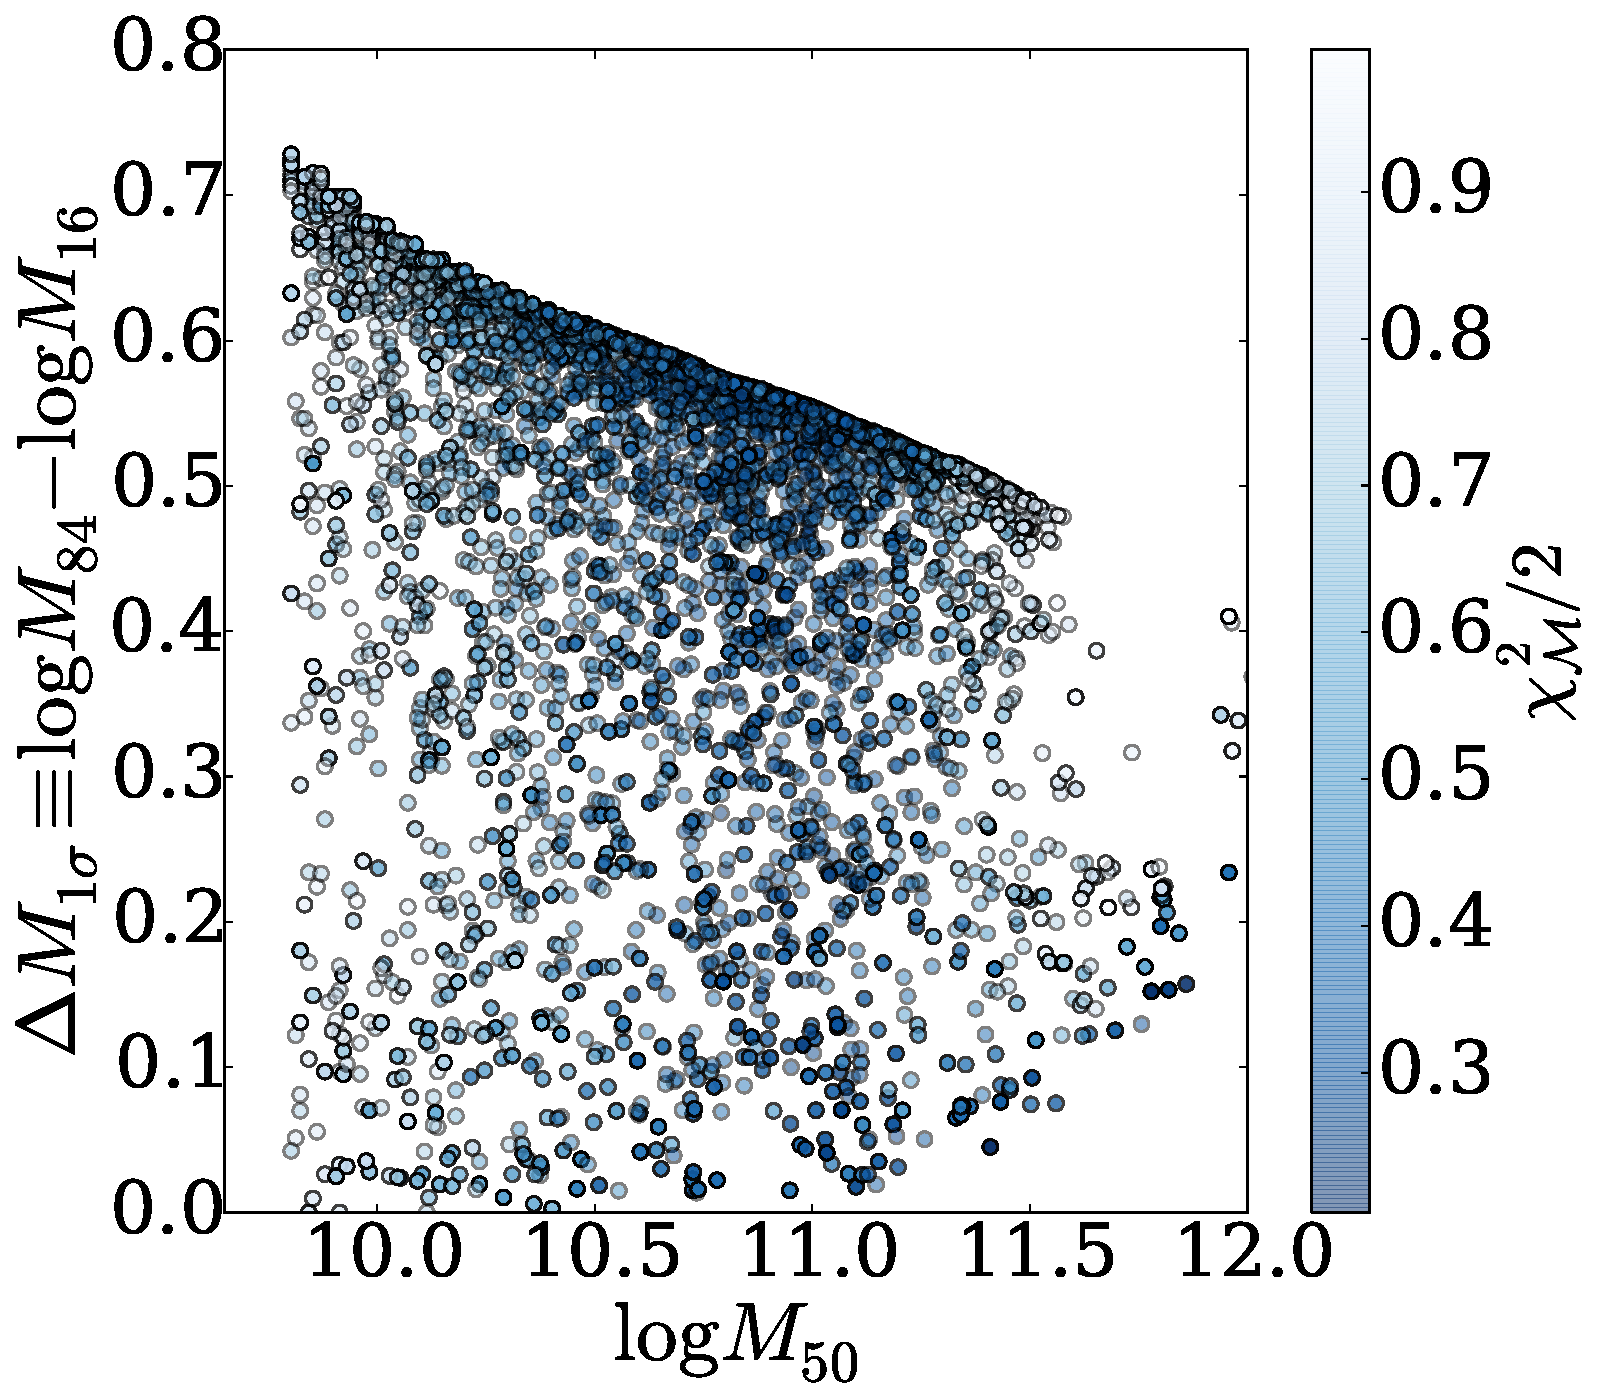
\includegraphics[width=0.47\textwidth]{fig4.pdf}
\caption{Median mass, $\log M_{50}$, and mass width $\Delta \log
  M_{1\sigma}=\log M_{84} - \log M_{16}$, for all models with low
  $\chi^2_{\mathcal{M}}/2 < 1.0$. 
  The median mass spans two orders of magnitude with a mean value
  around $10^{10.5}$\hMsun.   
  The mass width $\Delta \log M_{1\sigma}$ has a median of $0.3$ dex (a factor
  of $2$ in mass) with a maximum value of $0.7$ dex (a factor of
  5). This means that all models consistent with observations have a
  very narrow range in halo mass.}
\label{fig:mmed}
\end{figure}

\subsection{Median Halo Mass and Halo Mass Width within Models}

We now compute the median mass, $\log M_{50}$, and the $1\sigma$ halo mass
width, $\Delta \log M_{1\sigma} \equiv \log M_{84} - \log M_{16}$, of the
LAE hosting halos for each model  $\mathcal{M}$ (here $M_{p}$
represents the $p$ percentile of the mass distribution); $\log M_{50}$
and $M_{1\sigma}$ allow a direct comparison between our results and
previous results in the literature
\citep[e.g.][]{Hayashino2004,Gawiser2007,Ouchi2010,Bielby16} that used
a more simplified approach. 

In Fig. \ref{fig:mmed} we show the $\log M_{50}$-$\Delta \log M_{1\sigma}$
plane for the models selected to have $\chi^{2}_{\mathcal{M}}/2 < 1$,
which roughly correspond to the $1\sigma$ region in the posterior
distribution for the model parameters. The color encodes the
$\chi^{2}_{\mathcal{M}}/2$ value. The median mass has a wide distribution
spanning two orders of magnitude.

From this distribution we obtain $\log M_{50} = 10.5\pm 0.6$ or
equivalently $M_{50} = 3.16^{+9.34}_{-2.37}\times 10^{10}$\hMsun.  
The $1\sigma$ uncertainty for this median value is estimated from the
$16$ and $84$ percentile values in the $\log M_{50}$ distribution.  
This result is consistent with previous
 estimations of  the  median dark matter halo mass reported by
 \citet{Bielby16} ($\tilde{M}_{\mathrm h} = 10^{11.0\pm0.6}$),
 \citet{Gawiser07} ($\tilde{M}_{\mathrm h} = 10^{10.9\pm0.9}$) and
 \citet{Ouchi2010} ($\tilde{M}_{\mathrm h} =
 6.7^{+42.0}_{6.7}\times10^{10}$) using semi-analitical approaches.   

However, the same Figure \ref{fig:mmed} shows something 
that semi-analytical approaches were not able to predict.
The mass width, $\Delta \log M_{1\sigma}$, that is the width of the mass
distribution for a given model with fixed $\mmin$ and $\mmax$, has a
median value and $1\sigma$ uncertainty of $\Delta \log M_{1\sigma} =
0.55^{+0.11}_{-0.31}$ dex.
This means that the mass range for halos hosting LAEs is very narrow.
There is only a factor of $2$ to $4$ between the lower and upper mass
boundary.

Summarizing, the median mass could be anything in the range
$10^{9.5}$\hMsun\ and $10^{11.5}$\hMsun\ (a $2.0$ dex range), but the width is
highly constrained to be between $0.2$ and $0.6$ dex.  


In Fig. \ref{fig:corr} we show the computed
$ACF_{\mathcal{M}}$ of models with $\lmmin=0.5$ and different values
of $\dlm$. We can see that the clustering gets stronger for larger
values of \dlm. Nevertheless, due to the large impact of cosmic
variance at the volume of the current observations all the models  are
basically consistent within errors. The last result together with the
large Poissonian observational error in the ACF explain the current
difficulty to put tighter constrains in \lmmax\ in our model. 


\subsection{Constraining Dark matter halos mass  with cosmic variance}
Fig. \ref{fig:cosmicv0}  shows the  halo number distribution (HND) in
the  mock fields of the simulation for different models
$\mathcal{M}$. By simple inspection one can infer an increase in the
distribution with as \lmmin increase.  This trend is confirmed in
Fig. \ref{fig:cosmicv}  where we plot the central 1-$\sigma$ (blue
diamonds) and 2-$\sigma$  (red dots) widths  of the NDH as a function
of \lmmin. We particularly found that when we consider survey fields
of $\sim1{\rm deg^2}$, the central  1-$\sigma$ (2-$\sigma$) width of
the HND increases monotonically from 0.05dex (0.10dex) when
$\lmmin=9.5$ to 0.20dex (0.35dex) when $\lmmin=12.0$. The latter
result opens the possibility to constrain the \lmmin (as well as the
median mass) of LAEs by simply measure the width of the distribution
of observed LAE along several observational fields mapping $\sim1{\rm
  deg^2}$ in area and the observational depth determined by the NB479
filter. 



%*************************************************************************

\begin{figure}
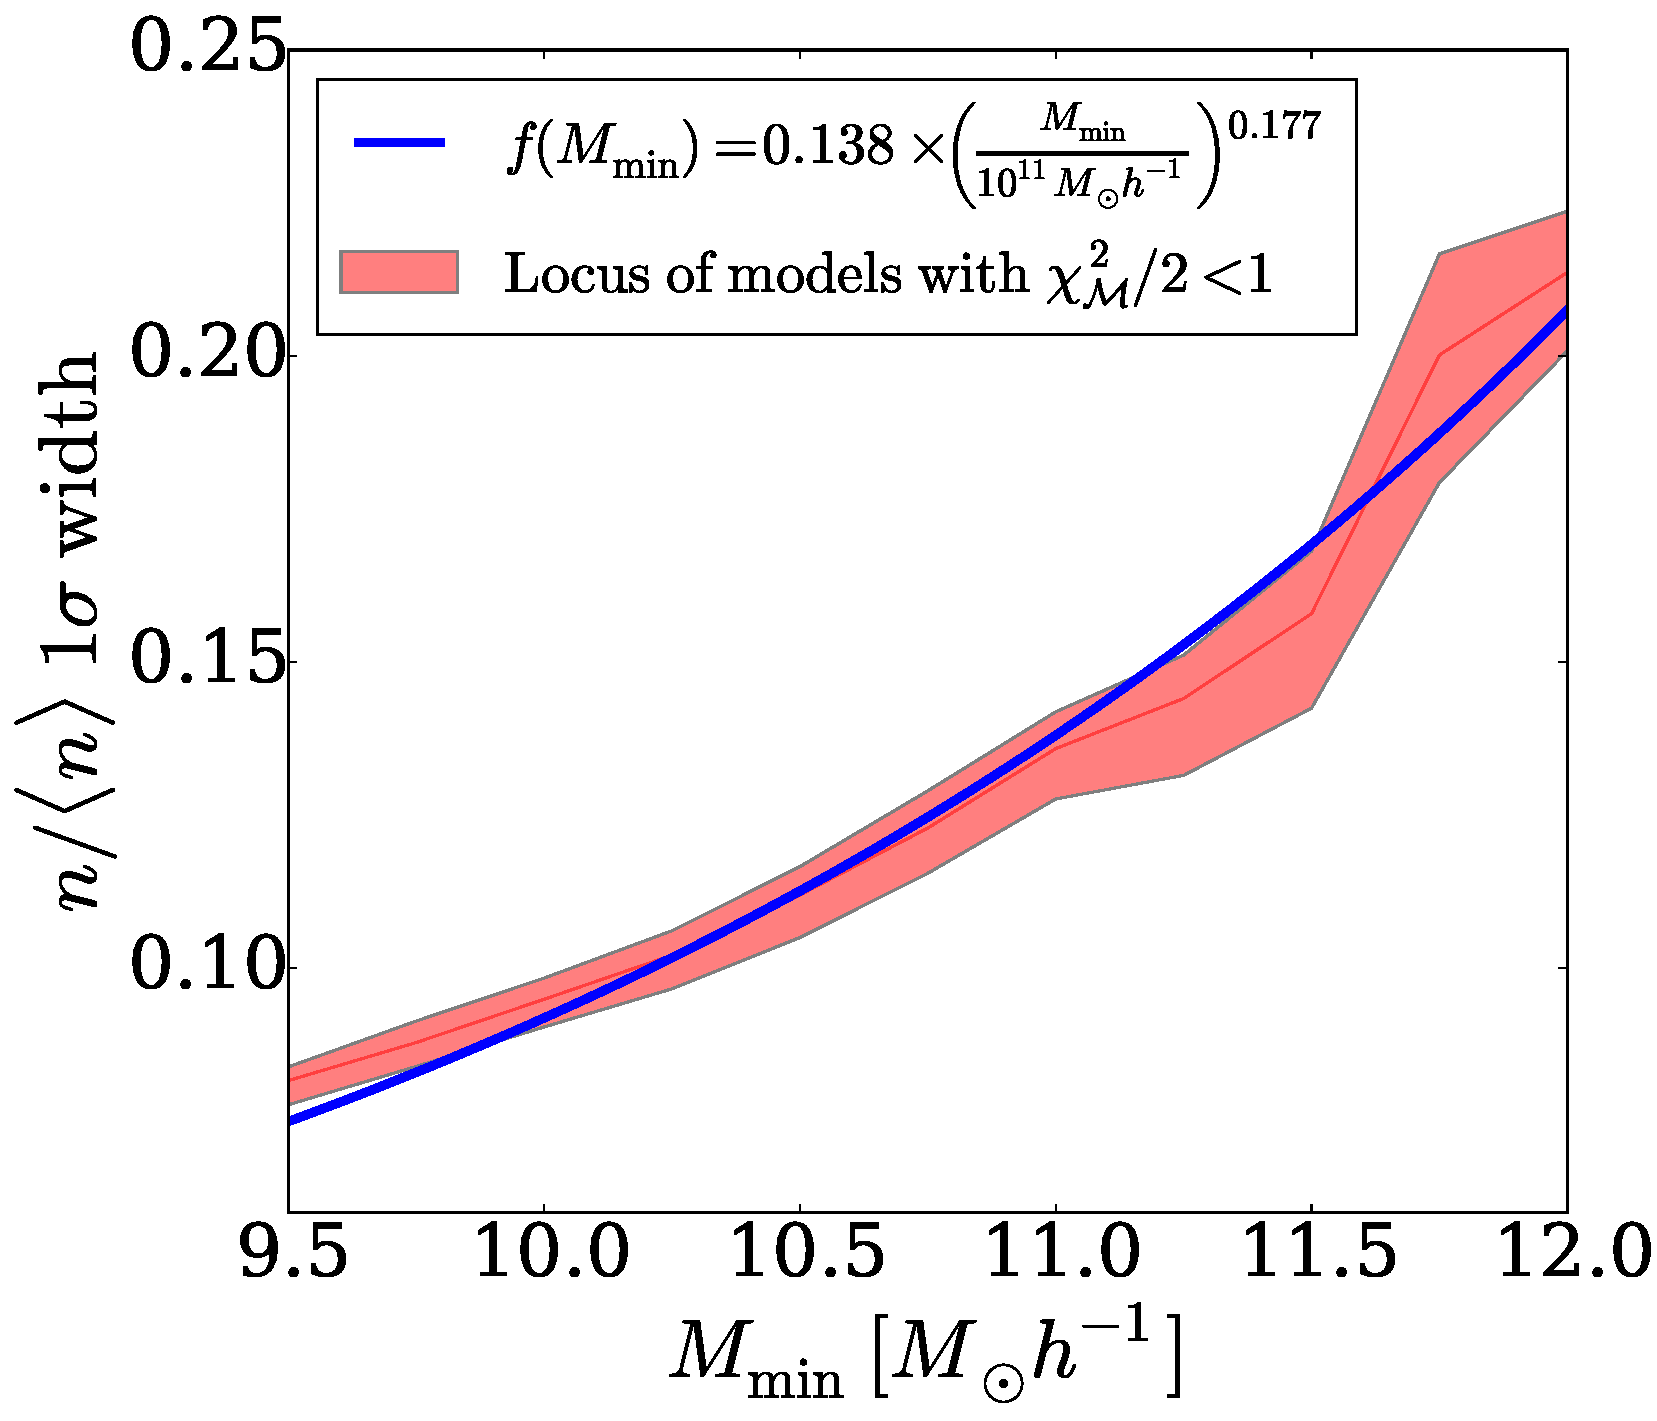
\includegraphics[width=0.49\textwidth]{fig6.pdf}
\caption{$1\sigma$ width of the number density distribution over the
  54 mock fields of the simulation as a function of \mmin. 
  Only the models that have a good match with observations
  ($\chi_{\mathcal M}/2 < 1$) are included.
  The strong dependence of $n/ \langle n\rangle$ with \mmin was
  parameterized as a power law with the parameters shown in the legend.
\label{fig:cosmicv}}
\end{figure}


\section{Conclusions}

In this letter we studied the impact of cosmic variance and
observational uncertainties in constraining the mass range and
occupation fraction of dark matter halos hosting  LAEs.   
To this end, we used the BolshoiP N-body simulation to construct  27
mock fields  with the same typical size  of observed fields at
$z=3.1$ ($\sim 1 {\rm deg^2}$).   
In our model a dark matter halo with mass in the range $M_{\rm
  min}<M_{\mathrm h}<M_{\rm   max}$ can only host one detectable LAE
at most.  
We explored the parameter space determined by \mmin\ and \mmax\ using
Monte Carlo Markov-Chain minimization to match the observed  ACF and
mean number density of LAEs.  

Our analysis allowed us to put weak constraints on $M_{\rm min}$,
$M_{\rm max}$ and $f_{\rm occ}$ where $10^{9.7}\hMsun\leq \log M_{\rm
  min}\leq 10^{11.2}\hMsun$, $10^{10.9}\hMsun\leq \log M_{\rm max}\leq
10^{13.0}\hMsun$ and $0.02\hMsun\leq f_{\rm occ}\leq 0.5$, spanning
three orders of magnitude in halo mass. 
Previous works\citep{Hayashino2004, Gawiser07,Ouchi2008,Bielby16} have
found typical masses within somehow narrower mass ranges ($\sim
10^{10.5}$-$10^{12}$).   
The main reason for our weaker constraints and large discrepancies
with previous works resides in the cosmic variance on the typical
field size in observations.  
A thorough exploration of cosmic variance impact as we present in this
letter had not been presented so far in the literature. 

Our analysis also allowed us to draw three results that can be used to
put tighter constraints on $M_{\rm min}$, $M_{\rm max}$ and $f_{\rm
  occ}$ once upcoming large LAE surveys, as the HETDEX project
\citep{Hetdex2011} and the HSC ultra deep survey, are available : 
\begin{enumerate}
\item $f_{\rm occ}$ and the median mass of LAEs are almost uniquely
  determined by $M_{\rm min}$ regardless of $M_{\rm max}$. \item
  measuring the width of the LAE number distribution function obtained
  over several fields of $\approx 1$ deg$^2$ one will be able to
  tightly constrain  $M_{\rm min}$, $M_{\rm med}$ and $f_{\rm occ}$ up
  to a factor of  2.  
\item  $M_{\rm max}$ drives the ACF strength at short angular
  distances ($<1\,\rm arcmin$), therefore precise measurements of the
  ACF at such scales are crucial to accurately determine \mmax. 
\end{enumerate}



\section*{Acknowledgments} 

JM acknowledges ``CONICYT-PCHA/doctorado Nacional para
extranjeros/2013-63130316'' for their PhD scholarship support.  

The authors gratefully acknowledge the Gauss Centre for Supercomputing
e.V. (\url{www.gauss-centre.eu}) and the Partnership for Advanced
Supercomputing in Europe (PRACE, \url{www.prace-ri.eu}) for funding the
MultiDark simulation project by providing computing time on the GCS
Supercomputer SuperMUC at Leibniz Supercomputing Centre (LRZ,
\url{www.lrz.de}). The Bolshoi simulations have been performed within the
Bolshoi project of the University of California High-Performance
AstroComputing Center (UC-HiPACC) and were run at the NASA Ames
Research Center. 


\bibliographystyle{apj}
\bibliography{references.bib}

\end{document}
